\documentclass[25pt, a0paper, portrait, margin=0mm, innermargin=15mm, blockverticalspace=15mm, colspace=15mm, subcolspace=8mm]{tikzposter}

\usepackage{amsmath}
\usepackage{epsf,graphicx,subfig}
\setcounter{tocdepth}{3}
\usepackage{xcolor}
\usepackage{lineno}
\usepackage[nolist]{acronym}
\usepackage{epsf,graphicx,subfig}
\usepackage{amssymb,amsmath}
\usepackage{tikz}
\usetikzlibrary{positioning}
\usepackage{todonotes}
\usepackage{standalone}
\usepackage{scalefnt}
\usepackage{url}

\usepackage{pgfplots}

\definecolor{udgColor}{RGB}{82,119,213}


\usetikzlibrary{arrows,backgrounds,shadows}

% define layers
    \pgfdeclarelayer{foreground}
    \pgfdeclarelayer{background}
    \pgfdeclarelayer{backgroundlayer} 
    \pgfdeclarelayer{notelayer}
% tell TikZ how to stack them (back to front)
    \pgfsetlayers{background,backgroundlayer,main,notelayer,foreground}


\title{\acs{sift} texture description for understanding breast ultrasound images}
\author{Joan Massich, Fabrice Meriaudeau, Melcior Sent{\'i}s, Sergi Ganau, Elsa~P{\'e}rez, Domenec Puig, Robert  Mart{\'i}, Arnau Oliver and Joan Mart{\'i}}

%\institute{contact author: sik@eia.udg.edu}
%\usetheme{Autumn}\usecolorstyle[colorPalette=BrownBlueOrange]{Germany}
\usetheme{Simple}
%\usecolorstyle[colorOne=udgColor]{Russia} 
\usecolorstyle[colorOne=udgColor]{Denmark} 

% This tex, loads the Breast GT pallete if is not defined.
% The document takes advantage of the xcolor package primitive 
% \def\@ifundefinedcolor#1{\@ifundefined{\string\color@#1}}
% therefore it xcolor package is needed or the definitions needs to be added.
% 
% TODO: 
% 	create a more generic script that checks if all the packages are there otherwise loads them.
%	or defines the missing primitive.
%   take a look at: \@ifpackageloaded{<name>}{<true>}{<false>}
% 					http://tex.stackexchange.com/questions/16199/test-if-a-package-or-package-option-is-loaded

\makeatletter
\newcommand{\colorprovide}[2]{%
  \@ifundefinedcolor{#1}{\colorlet{#1}{#2}}{}}

\newcommand{\defineColorWhenNoExist}[3]{%
  \@ifundefinedcolor{#1}{\definecolor{#1}{#2}{#3}}{}}
\makeatother

\defineColorWhenNoExist{bgColor}{rgb}{0.0000, 0.0000, 0.0000}
\defineColorWhenNoExist{boundaryColor}{rgb}{0.8784, 0.8784, 0.7529}
\defineColorWhenNoExist{chestWallColor}{rgb}{0.5294, 0.7843, 0.6078}
\defineColorWhenNoExist{fatColor}{rgb}{0.9804, 0.5882, 0.1176}
\defineColorWhenNoExist{fibroGlandColor}{rgb}{1.0000, 1.0000, 0.0000}
\defineColorWhenNoExist{lesionColor}{rgb}{1.0000, 0.2510, 0.0000}
\defineColorWhenNoExist{lungColor}{rgb}{0.2353, 0.6078, 0.8235}
\defineColorWhenNoExist{pectoralColor}{rgb}{0.6510, 0.3490, 1.0000}
\defineColorWhenNoExist{ribColor}{rgb}{0.0000, 0.4510, 0.1961}
\defineColorWhenNoExist{skinColor}{rgb}{0.9804, 0.7255, 0.7451}
\defineColorWhenNoExist{unkTissueColor}{rgb}{0.6000, 0.3020, 0.2510}


\begin{document}\maketitle
/home/sik/Work/escola/recerca/iwdm2014/paper/acronyms.tex

\graphicspath{{figures/paperFigures/}}
%\graphicspath{{figures/lowLevelConfMatrix/}}
\acresetall



\begin{columns} \column{0.45}

\block{Problem definition}{
xxxxxxxxxxxxxxxxxxxxxxxxxx
 
}

\block{xxxxxxxxxx}{
\begin{tikzfigure}[\acs{sift} space. (a) Projected space colored according to \acs{gt} tissue labeling. (b) $P(\bar{x}_a)$. (c) $P(\omega)$.]
\documentclass[border=2pt]{standalone}
\usepackage{tikz}
\usepackage{pgfplots,pgfplotstable}
\pgfplotsset{compat=1.4}
\usetikzlibrary{pgfplots.groupplots}

%\graphicspath{{../paperFigures/}}
% This tex, loads the Breast GT pallete if is not defined.
% The document takes advantage of the xcolor package primitive 
% \def\@ifundefinedcolor#1{\@ifundefined{\string\color@#1}}
% therefore it xcolor package is needed or the definitions needs to be added.
% 
% TODO: 
% 	create a more generic script that checks if all the packages are there otherwise loads them.
%	or defines the missing primitive.
%   take a look at: \@ifpackageloaded{<name>}{<true>}{<false>}
% 					http://tex.stackexchange.com/questions/16199/test-if-a-package-or-package-option-is-loaded

\makeatletter
\newcommand{\colorprovide}[2]{%
  \@ifundefinedcolor{#1}{\colorlet{#1}{#2}}{}}

\newcommand{\defineColorWhenNoExist}[3]{%
  \@ifundefinedcolor{#1}{\definecolor{#1}{#2}{#3}}{}}
\makeatother

\defineColorWhenNoExist{bgColor}{rgb}{0.0000, 0.0000, 0.0000}
\defineColorWhenNoExist{boundaryColor}{rgb}{0.8784, 0.8784, 0.7529}
\defineColorWhenNoExist{chestWallColor}{rgb}{0.5294, 0.7843, 0.6078}
\defineColorWhenNoExist{fatColor}{rgb}{0.9804, 0.5882, 0.1176}
\defineColorWhenNoExist{fibroGlandColor}{rgb}{1.0000, 1.0000, 0.0000}
\defineColorWhenNoExist{lesionColor}{rgb}{1.0000, 0.2510, 0.0000}
\defineColorWhenNoExist{lungColor}{rgb}{0.2353, 0.6078, 0.8235}
\defineColorWhenNoExist{pectoralColor}{rgb}{0.6510, 0.3490, 1.0000}
\defineColorWhenNoExist{ribColor}{rgb}{0.0000, 0.4510, 0.1961}
\defineColorWhenNoExist{skinColor}{rgb}{0.9804, 0.7255, 0.7451}
\defineColorWhenNoExist{unkTissueColor}{rgb}{0.6000, 0.3020, 0.2510}


\begin{document}

\pgfplotstableread[col sep=comma]{
Class, Occurrence, Pw
%-------------------------------------
Bg,     518738,	0.207
Lungs,  447153,	0.178
CWall,  134165,	0.054
Ribs,   22541, 	0.009
Pect,	  182468,	0.073
FGlan,  525238,	0.210
Fat,    413118,	0.165
Skin,   17732, 	0.007
Lsion,  163848,	0.065
Bound,  81082, 	0.032
}\occurrenceDataTable

\pgfplotscreateplotcyclelist{colorbrewer-RYB}{
{bgColor!50!black,fill=bgColor},
{lungColor!50!black,fill=lungColor},
{chestWallColor!50!black,fill=chestWallColor},
{ribColor!50!black,fill=ribColor},
{pectoralColor!50!black,fill=pectoralColor},
{fibroGlandColor!50!black,fill=fibroGlandColor},
{fatColor!50!black,fill=fatColor},
{skinColor!50!black,fill=skinColor},
{lesionColor!50!black,fill=lesionColor},
{boundaryColor!50!black,fill=boundaryColor},
}

\pgfplotsset{
    select row/.style={
        x filter/.code={\ifnum\coordindex=#1\else\def\pgfmathresult{}\fi}
    }
}

\newcommand\mySize{6cm} 

\begin{tikzpicture}
\begin{axis}[ 
              ybar=0pt,
              /pgf/bar shift=0pt,scale only axis,
              width=\mySize,
              ymin=0,
              xtick=\empty,
              tickpos=left,
              scaled y ticks=base 10:2,
              cycle list name=colorbrewer-RYB,
              bar width=14pt,
              ymajorgrids,
              font=\tiny,
              title=\small $P(\omega)$,
              name=pwAxis,
            ] 


\pgfplotsinvokeforeach  {0,...,9}{
  \addplot table [ x expr=\coordindex, select row=#1, y=Pw] {\occurrenceDataTable};
}
\end{axis}

\node at (pwAxis.south) 
      [ anchor=north,
        inner sep=0,
        yshift=-10pt,
%        draw,
        label=below:\small $P(\bar{x})$,
      ]{\includegraphics[height=\mySize]{siftOccurrences2}};
\end{tikzpicture}
\end{document}

\end{tikzfigure}
} 

\block{xxx}{
hello world !!
%\begin{tikzfigure}[Here is some caption]
%%\documentclass[border=2pt]{standalone}
\usepackage{tikz}
\usepackage{pgfplots}

% This tex, loads the Breast GT pallete if is not defined.
% The document takes advantage of the xcolor package primitive 
% \def\@ifundefinedcolor#1{\@ifundefined{\string\color@#1}}
% therefore it xcolor package is needed or the definitions needs to be added.
% 
% TODO: 
% 	create a more generic script that checks if all the packages are there otherwise loads them.
%	or defines the missing primitive.
%   take a look at: \@ifpackageloaded{<name>}{<true>}{<false>}
% 					http://tex.stackexchange.com/questions/16199/test-if-a-package-or-package-option-is-loaded

\makeatletter
\newcommand{\colorprovide}[2]{%
  \@ifundefinedcolor{#1}{\colorlet{#1}{#2}}{}}

\newcommand{\defineColorWhenNoExist}[3]{%
  \@ifundefinedcolor{#1}{\definecolor{#1}{#2}{#3}}{}}
\makeatother

\defineColorWhenNoExist{bgColor}{rgb}{0.0000, 0.0000, 0.0000}
\defineColorWhenNoExist{boundaryColor}{rgb}{0.8784, 0.8784, 0.7529}
\defineColorWhenNoExist{chestWallColor}{rgb}{0.5294, 0.7843, 0.6078}
\defineColorWhenNoExist{fatColor}{rgb}{0.9804, 0.5882, 0.1176}
\defineColorWhenNoExist{fibroGlandColor}{rgb}{1.0000, 1.0000, 0.0000}
\defineColorWhenNoExist{lesionColor}{rgb}{1.0000, 0.2510, 0.0000}
\defineColorWhenNoExist{lungColor}{rgb}{0.2353, 0.6078, 0.8235}
\defineColorWhenNoExist{pectoralColor}{rgb}{0.6510, 0.3490, 1.0000}
\defineColorWhenNoExist{ribColor}{rgb}{0.0000, 0.4510, 0.1961}
\defineColorWhenNoExist{skinColor}{rgb}{0.9804, 0.7255, 0.7451}
\defineColorWhenNoExist{unkTissueColor}{rgb}{0.6000, 0.3020, 0.2510}

\begin{document}

\newcommand\confMatrixSize{20cm}
\newcommand\gtLabelDistance{0.3cm}

\pgfplotsset{
	myStyleCommon/.append style={	width=\confMatrixSize,height=\confMatrixSize,
									scale only axis,
									xlabel={Estimated Class},
								    ylabel={Actual Class},
								    yticklabels={},
								    xticklabels={},
									xticklabel pos=right,
									xlabel near ticks,
									xtick={1.5,2.5,...,9.5},
									ytick={1.5,2.5,...,9.5},
									grid,
      }
}

\pgfplotsset{
	confMatrix/.append	style={	myStyleCommon,
								axis on top,
								colormap/jet,
								point meta min=0,
								point meta max=1,
								xmin=0.5,
								xmax=10.5,
								y dir=reverse,
								ymin=0.5,
								ymax=10.5,
							  }
}
\pgfplotsset{							  
	gtLabelsAxis/.append style={myStyleCommon,
								axis lines=none,
								colormap={labelsGT}{color(0cm)=(bgColor);
					 								color(1cm)=(lungColor);	
					 								color(2cm)=(chestWallColor);
										 			color(3cm)=(ribColor);
										 			color(4cm)=(pectoralColor);
										 			color(5cm)=(fibroGlandColor); 
										 			color(6cm)=(fatColor); 
					 								color(7cm)=(skinColor);    
								 					color(8cm)=(lesionColor);
							 						color(9cm)=(boundaryColor); 
					 								color(10cm)=(unkTissueColor); 
					 								},
							    point meta min=0,
							    point meta max=10,
							    xmin=-0.5,xmax=9.5,
							    height=0cm,
							  }				  
}
\tikzstyle{gtLabelsPlotStyle}=[scatter,only marks,mark=square*,mark size=5pt,domain=0:9,samples at={0,...,9}]
\tikzstyle{stdDrawingStyle} = [scatter, only marks, mark size=4pt]

\begin{tikzpicture}
\begin{axis}[confMatrix,name=siftConfMatrix]
            \addplot graphics [xmin=0.5,xmax=10.5,ymin=0.5,ymax=10.5] {LowLevelSIFTConfusionMatrixMean.png};

			\addplot[stdDrawingStyle,
					 % we use ’point meta’ as color data...
					point meta=\thisrow{siftStd},
					% ... therefore, we can’t use it as argument for nodes near coords ..
					% ... look how to print the numbers at pgfplotstable.pdf manual
			        nodes near coords*={$
				        				\pgfmathprintnumber[fixed,precision=0]{\meanVal}
				        				\pm
				        				\pgfmathprintnumber[fixed,precision=1]{\stdVal}
				        				$},
			        % ... which requires to define a visualization dependency:
           			visualization depends on={100*\thisrow{siftMean} \as \meanVal},
           			visualization depends on={100*\thisrow{siftStd} \as \stdVal},
					]
					table[	y=actualClass,
							x=estimatedClass,
 						 ]{lowLevelFeaturesConfusion.dat};
\end{axis}

\begin{axis}[gtLabelsAxis,
			 at=(siftConfMatrix.north),anchor=south,
			 yshift=\gtLabelDistance,
			 name=xGTLabelsSIFT,
			 ]
			\addplot [gtLabelsPlotStyle,point meta=x] {0};
\end{axis}
 
\begin{axis}[	gtLabelsAxis,
				rotate=-90,yshift=-\gtLabelDistance,
			 	name=yGTLabelsSIFT,
			 ]
			\addplot [gtLabelsPlotStyle,point meta=x] {0};   	
\end{axis}

\end{tikzpicture}


\end{document}

%  
%\end{tikzfigure}
\begin{tikzfigure}[\acs{sift} space. (a) Projected space colored according to \acs{gt} tissue labeling. (b) $P(\bar{x}_a)$. (c) $P(\omega)$.]
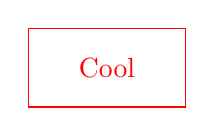
\begin{tikzpicture}
\draw [color=red] (0,0) rectangle (2,1) node [midway] {Cool};
\end{tikzpicture}
\end{tikzfigure}
}





\end{columns}
\block[titleoffsety=-1cm,bodyoffsety=-1cm]{Sample document}{This poster...}
%\note[targetoffsetx=24cm, targetoffsety=-9cm,radius=8cm,width=.75\textwidth,innersep=.4cm]{You can...}
\note[targetoffsetx=0cm,targetoffsety=-9cm,radius=8cm,width=.5\textwidth,innersep=.4cm]{You can...}
\end{document}
